\documentclass[11pt,a4paper]{article}
\usepackage[T1]{fontenc}
\usepackage[left=2cm, right=2cm, top=2cm, bottom=2cm]{geometry}
\usepackage{graphicx}
\usepackage{mathtools}
\usepackage{amssymb}
\usepackage{amsthm}
\usepackage{thmtools}
\usepackage{xcolor}
\usepackage{nameref}
\usepackage[colorlinks=true, linkcolor=blue, citecolor=cyan]{hyperref}
\usepackage{natbib} 
\usepackage{tkz-graph}
\usepackage{placeins}


\newcommand{\grad}{\operatorname{grad}}
\newcommand{\curl}{\operatorname{curl}}
\renewcommand{\div}{\operatorname{div}}
\newcommand{\img}{\operatorname{img}}
\renewcommand{\span}{\operatorname{span}}
\newcommand{\Z}{\mathbb{Z}}
\newcommand{\tile}[1]{\fbox{{#1}}}

\usepackage{tikz}
\usepackage{xparse}

\NewDocumentCommand{\T}{>{\SplitList{,}}m}{%
	\ProcessList{#1}{\PlaceOnSquare}%
}

\newcommand{\PlaceOnSquare}[4]{%
	\tikz[baseline=(sq.base),scale=0.6]{%
		\node[draw,minimum size=1cm,inner sep=0pt] (sq) {};
		\node[font=\tiny,above] at (sq.north) {#1};
		\node[font=\tiny,right] at (sq.east)  {#2};
		\node[font=\tiny,below] at (sq.south) {#3};
		\node[font=\tiny,left]  at (sq.west)  {#4};
	}%
}



\theoremstyle{definition}
\newtheorem{definition}{Definition}


\theoremstyle{remark}
\newtheorem{remark}{Remark}

\title{Some topological insights to the tiling problem on $ \Z^d $}
\author{Ali Fele Paranj}


\theoremstyle{definition}
\newtheorem{theorem}{Theorem}


\begin{document}
	
	\maketitle
	\begin{abstract}
		In this document I will translates some of the problems in tiling self-assembly to the language of analysis and topology, hoping to open the was for using ergodic theory and other interesting analytical tools. 
	\end{abstract}
	
	
	\section{Introduction}
	
	Let's consider the set of all 2D tiles over the final alphabet $\Sigma$. The set of all such possible tilings is 
	$$ \Sigma^{\mathbb{Z}^2}, $$
	which is the same as the set of all functions from $\mathbb{Z}^2$ to $\Sigma$. 
	
	First, observe that since the alphabet is finite, assuming that it has $N$ elements, then one can write $[n] = \{1,2,3,\cdots,n\}$ in place of $\Sigma$. As far as the set structure of $\Sigma$ is considered, it is fine to do so. However, seeing these two spaces as topological spaces, one automatically assumes a discrete topology over the set $\Sigma$, however, in the case of $[n]$ one automatically assumes that 2 is "close" to 1 and 3 and far from $n$. So we might exploit this topological property of the alphabet set in deciding which tilling is plausible and which is not: based on their gluing structure, that a tile of certain type is willing to be close to the tiles of other type. Then one can possibly encode the plausible tiles as functions that are continuous given the topology of their domain $\mathbb{Z}^2$ and their range $\Sigma$. For more about the intuition behind the method see my notes in this \href{https://github.com/alifele/Lecture-Notes/blob/main/Scientific%20Notes/Some%20Intuitions%20on%20Continuous%20Maps/GraphHomologyAndCohomology.pdf}{link}.
	
	
	\section{Simple Setup}
	Define the $ d_1 $ metric on $ \Z^2 $, where
	\[ d_1\left( (n_1,n_2), (m_1,m_2) \right) = |n_1-n_2| + |m_1-m_2|. \]
	This will induce the topology where the smallest open balls are the Moor neighborhoods (see the first chapter of my \href{https://open.library.ubc.ca/soa/cIRcle/collections/ubctheses/24/items/1.0449873}{thesis} for more on this.) Also assume that we have three types of tiles $ \{ \tile{A}, \tile{B}, \tile{C} \}. $ Assuming that every tile can sit with itself (this can be relaxed later by constructing large enough product space), then the notion of ``certain tiles want to it close to certain other tiles'' will induce a partition on the set of tiles (because it is a equivalence relation). Consider the topology whose sub-basis is this partition of the set. The following figure demonstrates this partition.
	
	\begin{figure}[h!]
	\centering
	
	
	\tikzset{every picture/.style={line width=0.75pt}} %set default line width to 0.75pt        
	
	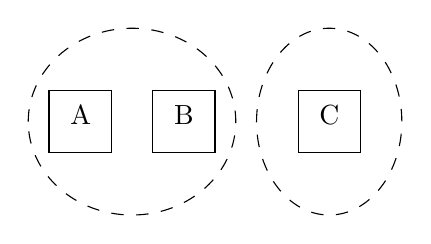
\begin{tikzpicture}[x=0.75pt,y=0.75pt,yscale=-1,xscale=1]
		%uncomment if require: \path (0,300); %set diagram left start at 0, and has height of 300
		
		%Shape: Square [id:dp45846669475066437] 
		\draw   (180,80) -- (210,80) -- (210,110) -- (180,110) -- cycle ;
		%Shape: Square [id:dp8694832240743474] 
		\draw   (230,80) -- (260,80) -- (260,110) -- (230,110) -- cycle ;
		%Shape: Square [id:dp9643149276555201] 
		\draw   (300,80) -- (330,80) -- (330,110) -- (300,110) -- cycle ;
		%Shape: Ellipse [id:dp7472268647554123] 
		\draw  [dash pattern={on 4.5pt off 4.5pt}] (170,95) .. controls (170,70.15) and (192.39,50) .. (220,50) .. controls (247.61,50) and (270,70.15) .. (270,95) .. controls (270,119.85) and (247.61,140) .. (220,140) .. controls (192.39,140) and (170,119.85) .. (170,95) -- cycle ;
		%Shape: Ellipse [id:dp9372300796607134] 
		\draw  [dash pattern={on 4.5pt off 4.5pt}] (280,95) .. controls (280,70.15) and (295.67,50) .. (315,50) .. controls (334.33,50) and (350,70.15) .. (350,95) .. controls (350,119.85) and (334.33,140) .. (315,140) .. controls (295.67,140) and (280,119.85) .. (280,95) -- cycle ;
		
		% Text Node
		\draw (189,86) node [anchor=north west][inner sep=0.75pt]   [align=left] {A};
		% Text Node
		\draw (239,86) node [anchor=north west][inner sep=0.75pt]   [align=left] {B};
		% Text Node
		\draw (309,86) node [anchor=north west][inner sep=0.75pt]   [align=left] {C};
		
		
	\end{tikzpicture}
\end{figure}
	
	Given this ``topology'' on the set of possible tiles, then the following demonstrates two tilings, where the one on the left is a valid tiling, but the one on the right is not a valid tiling.
	
	\begin{figure}[h!]
	\centering
	
	
	\tikzset{every picture/.style={line width=0.75pt}} %set default line width to 0.75pt        
	
	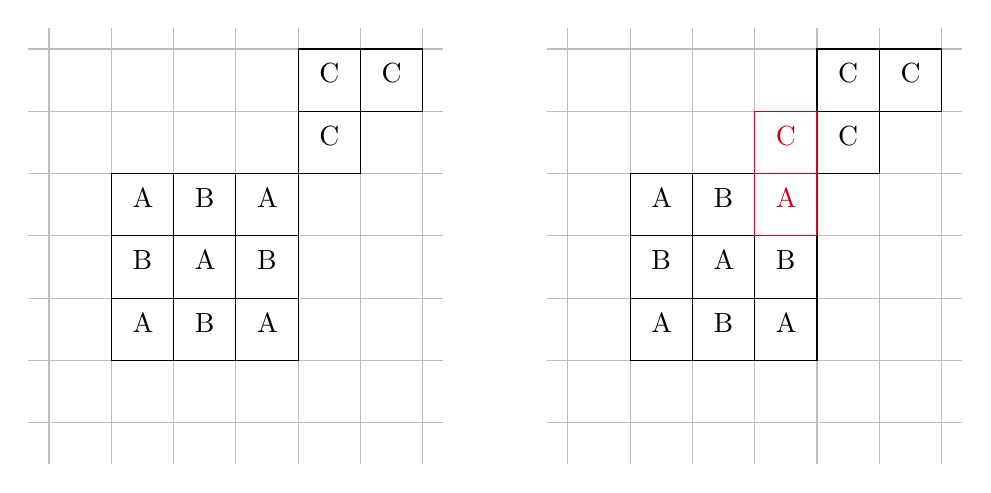
\begin{tikzpicture}[x=0.75pt,y=0.75pt,yscale=-1,xscale=1]
		%uncomment if require: \path (0,300); %set diagram left start at 0, and has height of 300
		
		%Straight Lines [id:da35045523066874695] 
		\draw [color={rgb, 255:red, 190; green, 188; blue, 188 }  ,draw opacity=1 ]   (60,40) -- (60,250) ;
		%Straight Lines [id:da340132848719611] 
		\draw [color={rgb, 255:red, 190; green, 188; blue, 188 }  ,draw opacity=1 ]   (90,40) -- (90,250) ;
		%Straight Lines [id:da9930602253194404] 
		\draw [color={rgb, 255:red, 190; green, 188; blue, 188 }  ,draw opacity=1 ]   (120,40) -- (120,250) ;
		%Straight Lines [id:da673508591738556] 
		\draw [color={rgb, 255:red, 190; green, 188; blue, 188 }  ,draw opacity=1 ]   (150,40) -- (150,250) ;
		%Straight Lines [id:da419114194150617] 
		\draw [color={rgb, 255:red, 190; green, 188; blue, 188 }  ,draw opacity=1 ]   (180,40) -- (180,250) ;
		%Straight Lines [id:da5545224299809445] 
		\draw [color={rgb, 255:red, 190; green, 188; blue, 188 }  ,draw opacity=1 ]   (210,40) -- (210,250) ;
		%Straight Lines [id:da6684800824274905] 
		\draw [color={rgb, 255:red, 190; green, 188; blue, 188 }  ,draw opacity=1 ]   (50,50) -- (250,50) ;
		%Straight Lines [id:da019342059581128557] 
		\draw [color={rgb, 255:red, 190; green, 188; blue, 188 }  ,draw opacity=1 ]   (240,40) -- (240,250) ;
		%Straight Lines [id:da9329975150298714] 
		\draw [color={rgb, 255:red, 190; green, 188; blue, 188 }  ,draw opacity=1 ]   (50,80) -- (250,80) ;
		%Straight Lines [id:da5923754330081309] 
		\draw [color={rgb, 255:red, 190; green, 188; blue, 188 }  ,draw opacity=1 ]   (50,110) -- (250,110) ;
		%Straight Lines [id:da3014815129266917] 
		\draw [color={rgb, 255:red, 190; green, 188; blue, 188 }  ,draw opacity=1 ]   (50,140) -- (250,140) ;
		%Straight Lines [id:da9700279192389916] 
		\draw [color={rgb, 255:red, 190; green, 188; blue, 188 }  ,draw opacity=1 ]   (50,170) -- (250,170) ;
		%Straight Lines [id:da6736918804400827] 
		\draw [color={rgb, 255:red, 190; green, 188; blue, 188 }  ,draw opacity=1 ]   (50,200) -- (250,200) ;
		%Straight Lines [id:da05640786705782641] 
		\draw [color={rgb, 255:red, 190; green, 188; blue, 188 }  ,draw opacity=1 ]   (50,230) -- (250,230) ;
		%Shape: Square [id:dp5803031662244053] 
		\draw   (120,140) -- (150,140) -- (150,170) -- (120,170) -- cycle ;
		
		%Shape: Square [id:dp9196458885257819] 
		\draw   (150,110) -- (180,110) -- (180,140) -- (150,140) -- cycle ;
		
		%Shape: Square [id:dp2648572079254672] 
		\draw   (150,170) -- (180,170) -- (180,200) -- (150,200) -- cycle ;
		
		%Shape: Square [id:dp5425673607779279] 
		\draw   (90,170) -- (120,170) -- (120,200) -- (90,200) -- cycle ;
		
		%Shape: Square [id:dp18348530459906254] 
		\draw   (90,110) -- (120,110) -- (120,140) -- (90,140) -- cycle ;
		
		%Shape: Square [id:dp8856504410510044] 
		\draw   (120,110) -- (150,110) -- (150,140) -- (120,140) -- cycle ;
		
		%Shape: Square [id:dp1873507618967537] 
		\draw   (90,140) -- (120,140) -- (120,170) -- (90,170) -- cycle ;
		
		%Shape: Square [id:dp022117374983126603] 
		\draw   (150,140) -- (180,140) -- (180,170) -- (150,170) -- cycle ;
		
		%Shape: Square [id:dp1634547289103776] 
		\draw   (120,170) -- (150,170) -- (150,200) -- (120,200) -- cycle ;
		
		%Shape: Square [id:dp36442727347773063] 
		\draw   (180,50) -- (210,50) -- (210,80) -- (180,80) -- cycle ;
		%Shape: Square [id:dp5330652912981374] 
		\draw   (210,50) -- (240,50) -- (240,80) -- (210,80) -- cycle ;
		%Shape: Square [id:dp4661865144958631] 
		\draw   (180,80) -- (210,80) -- (210,110) -- (180,110) -- cycle ;
		%Straight Lines [id:da6005649012467171] 
		\draw [color={rgb, 255:red, 190; green, 188; blue, 188 }  ,draw opacity=1 ]   (310,40) -- (310,250) ;
		%Straight Lines [id:da04035283072064799] 
		\draw [color={rgb, 255:red, 190; green, 188; blue, 188 }  ,draw opacity=1 ]   (340,40) -- (340,250) ;
		%Straight Lines [id:da671906501011724] 
		\draw [color={rgb, 255:red, 190; green, 188; blue, 188 }  ,draw opacity=1 ]   (370,40) -- (370,250) ;
		%Straight Lines [id:da49929915066743213] 
		\draw [color={rgb, 255:red, 190; green, 188; blue, 188 }  ,draw opacity=1 ]   (400,40) -- (400,250) ;
		%Straight Lines [id:da6124906908305024] 
		\draw [color={rgb, 255:red, 190; green, 188; blue, 188 }  ,draw opacity=1 ]   (430,40) -- (430,250) ;
		%Straight Lines [id:da17945370773484437] 
		\draw [color={rgb, 255:red, 190; green, 188; blue, 188 }  ,draw opacity=1 ]   (460,40) -- (460,250) ;
		%Straight Lines [id:da6328554243047342] 
		\draw [color={rgb, 255:red, 190; green, 188; blue, 188 }  ,draw opacity=1 ]   (300,50) -- (500,50) ;
		%Straight Lines [id:da6688510350866759] 
		\draw [color={rgb, 255:red, 190; green, 188; blue, 188 }  ,draw opacity=1 ]   (490,40) -- (490,250) ;
		%Straight Lines [id:da612235496519943] 
		\draw [color={rgb, 255:red, 190; green, 188; blue, 188 }  ,draw opacity=1 ]   (300,80) -- (500,80) ;
		%Straight Lines [id:da4514565784776753] 
		\draw [color={rgb, 255:red, 190; green, 188; blue, 188 }  ,draw opacity=1 ]   (300,110) -- (500,110) ;
		%Straight Lines [id:da9360017779771976] 
		\draw [color={rgb, 255:red, 190; green, 188; blue, 188 }  ,draw opacity=1 ]   (300,140) -- (500,140) ;
		%Straight Lines [id:da8873772965675616] 
		\draw [color={rgb, 255:red, 190; green, 188; blue, 188 }  ,draw opacity=1 ]   (300,170) -- (500,170) ;
		%Straight Lines [id:da749590494256885] 
		\draw [color={rgb, 255:red, 190; green, 188; blue, 188 }  ,draw opacity=1 ]   (300,200) -- (500,200) ;
		%Straight Lines [id:da974945622190988] 
		\draw [color={rgb, 255:red, 190; green, 188; blue, 188 }  ,draw opacity=1 ]   (300,230) -- (500,230) ;
		%Shape: Square [id:dp3113813487928936] 
		\draw   (370,140) -- (400,140) -- (400,170) -- (370,170) -- cycle ;
		
		%Shape: Square [id:dp6490479518389014] 
		\draw   (400,170) -- (430,170) -- (430,200) -- (400,200) -- cycle ;
		
		%Shape: Square [id:dp39859172546594845] 
		\draw   (340,170) -- (370,170) -- (370,200) -- (340,200) -- cycle ;
		
		%Shape: Square [id:dp2225864237176991] 
		\draw   (340,110) -- (370,110) -- (370,140) -- (340,140) -- cycle ;
		
		%Shape: Square [id:dp7921412678362084] 
		\draw   (370,110) -- (400,110) -- (400,140) -- (370,140) -- cycle ;
		
		%Shape: Square [id:dp6449792794581529] 
		\draw   (340,140) -- (370,140) -- (370,170) -- (340,170) -- cycle ;
		
		%Shape: Square [id:dp10628620173289283] 
		\draw   (400,140) -- (430,140) -- (430,170) -- (400,170) -- cycle ;
		
		%Shape: Square [id:dp14519260765485775] 
		\draw   (370,170) -- (400,170) -- (400,200) -- (370,200) -- cycle ;
		
		%Shape: Square [id:dp3804583310680284] 
		\draw   (430,50) -- (460,50) -- (460,80) -- (430,80) -- cycle ;
		%Shape: Square [id:dp8462651005127663] 
		\draw   (460,50) -- (490,50) -- (490,80) -- (460,80) -- cycle ;
		%Shape: Square [id:dp23845380767750257] 
		\draw   (430,80) -- (460,80) -- (460,110) -- (430,110) -- cycle ;
		%Shape: Square [id:dp21222113434847067] 
		\draw  [color={rgb, 255:red, 208; green, 2; blue, 27 }  ,draw opacity=1 ] (400,80) -- (430,80) -- (430,110) -- (400,110) -- cycle ;
		%Shape: Square [id:dp188598855194557] 
		\draw  [color={rgb, 255:red, 208; green, 2; blue, 27 }  ,draw opacity=1 ] (400,110) -- (430,110) -- (430,140) -- (400,140) -- cycle ;
		
		
		% Text Node
		\draw (129,146) node [anchor=north west][inner sep=0.75pt]   [align=left] {A};
		% Text Node
		\draw (159,116) node [anchor=north west][inner sep=0.75pt]   [align=left] {A};
		% Text Node
		\draw (159,176) node [anchor=north west][inner sep=0.75pt]   [align=left] {A};
		% Text Node
		\draw (99,176) node [anchor=north west][inner sep=0.75pt]   [align=left] {A};
		% Text Node
		\draw (99,116) node [anchor=north west][inner sep=0.75pt]   [align=left] {A};
		% Text Node
		\draw (129,116) node [anchor=north west][inner sep=0.75pt]   [align=left] {B};
		% Text Node
		\draw (99,146) node [anchor=north west][inner sep=0.75pt]   [align=left] {B};
		% Text Node
		\draw (159,146) node [anchor=north west][inner sep=0.75pt]   [align=left] {B};
		% Text Node
		\draw (129,176) node [anchor=north west][inner sep=0.75pt]   [align=left] {B};
		% Text Node
		\draw (189,56) node [anchor=north west][inner sep=0.75pt]   [align=left] {C};
		% Text Node
		\draw (219,56) node [anchor=north west][inner sep=0.75pt]   [align=left] {C};
		% Text Node
		\draw (189,86) node [anchor=north west][inner sep=0.75pt]   [align=left] {C};
		% Text Node
		\draw (439,56) node [anchor=north west][inner sep=0.75pt]   [align=left] {C};
		% Text Node
		\draw (469,56) node [anchor=north west][inner sep=0.75pt]   [align=left] {C};
		% Text Node
		\draw (439,86) node [anchor=north west][inner sep=0.75pt]   [align=left] {C};
		% Text Node
		\draw (379,176) node [anchor=north west][inner sep=0.75pt]   [align=left] {B};
		% Text Node
		\draw (409,146) node [anchor=north west][inner sep=0.75pt]   [align=left] {B};
		% Text Node
		\draw (349,146) node [anchor=north west][inner sep=0.75pt]   [align=left] {B};
		% Text Node
		\draw (379,116) node [anchor=north west][inner sep=0.75pt]   [align=left] {B};
		% Text Node
		\draw (349,116) node [anchor=north west][inner sep=0.75pt]   [align=left] {A};
		% Text Node
		\draw (349,176) node [anchor=north west][inner sep=0.75pt]   [align=left] {A};
		% Text Node
		\draw (409,176) node [anchor=north west][inner sep=0.75pt]   [align=left] {A};
		% Text Node
		\draw (409,116) node [anchor=north west][inner sep=0.75pt]   [align=left] {\textcolor[rgb]{0.82,0.01,0.11}{A}};
		% Text Node
		\draw (379,146) node [anchor=north west][inner sep=0.75pt]   [align=left] {A};
		% Text Node
		\draw (409,86) node [anchor=north west][inner sep=0.75pt]  [color={rgb, 255:red, 208; green, 2; blue, 27 }  ,opacity=1 ] [align=left] {C};
		
		
	\end{tikzpicture}
\end{figure}
	
	\FloatBarrier
	
	So given the intuition above, one can come up with the following theorem
	
	\begin{theorem}
		In the tiling problem above, a tiling is valid, if and only if its corresponding tiling function is continuous.
	\end{theorem}
	
	
	
	\begin{remark}
		One possible way to formulate this is to assume a discrete topology on $ \Z^2 $, which will force every tiling map to be continuous. However, then, the tiling maps corresponding to valid tiling will precisely be the open maps (the maps that the image of open sets are open sets). 
	\end{remark}
	
	
	\section{Tiles with Glue}
	
	In the example above, we only considered some that some of them want to sit with some other ones and do not sit with certain other ones. However, the way that the tiling problem is formulated in the literature is to assume tiles with different combination of glue values on the sides. I think I can convert this problem to the one similar to above, by considering a sufficiently large product space that captures glue-glue interactions. I know that each glue glue interaction can be captured by a matrix, but I an not certain how to define approporiate topology to convert this formulation to the one similar to above.
	
	
	\subsection{One Possible Formulation}
	Let's assume that the set of all possible glues types is given as alphabet $ G $. For instance, if we have 3 types of glue, then one has $ G = \{g_1,g_2,g_3\} $. Assuming that we work in a 2d grid, consider $ T = G^4 $ or equivalently the set of all strings composed of alphabet in $ G $. For instance, if $ G $ is as given above, then
	\[ \mathcal{T} = \{ g_1g_1g_1g_1,\ g_1g_1g_1g_2,\ g_1g_1g_2g_1,\cdots, g_3g_3g_3g_3. \} \]
	This is the set of all possible tiles. Note that given a combination of glue alphabet, we might not have all of the tiles in $ \mathcal{T} $. For instance, for $ G $ as given above, in one problem we might have only two tiles. For instance:
	\begin{figure}[h!]
	\centering
	
	
	\tikzset{every picture/.style={line width=0.75pt}} %set default line width to 0.75pt        
	
	\begin{tikzpicture}[x=0.75pt,y=0.75pt,yscale=-1,xscale=1]
		%uncomment if require: \path (0,300); %set diagram left start at 0, and has height of 300
		
		%Shape: Square [id:dp14909296198340416] 
		\draw   (170,90) -- (220,90) -- (220,140) -- (170,140) -- cycle ;
		%Shape: Square [id:dp0035098982066744666] 
		\draw   (283,90) -- (333,90) -- (333,140) -- (283,140) -- cycle ;
		
		% Text Node
		\draw (191,76.4) node [anchor=north west][inner sep=0.75pt]  [font=\scriptsize]  {$g_{1}$};
		% Text Node
		\draw (223,106.4) node [anchor=north west][inner sep=0.75pt]  [font=\scriptsize]  {$g_{1}$};
		% Text Node
		\draw (191,138.4) node [anchor=north west][inner sep=0.75pt]  [font=\scriptsize]  {$g_{2}$};
		% Text Node
		\draw (156,106.4) node [anchor=north west][inner sep=0.75pt]  [font=\scriptsize]  {$g_{2}$};
		% Text Node
		\draw (304,76.4) node [anchor=north west][inner sep=0.75pt]  [font=\scriptsize]  {$g_{2}$};
		% Text Node
		\draw (336,106.4) node [anchor=north west][inner sep=0.75pt]  [font=\scriptsize]  {$g_{3}$};
		% Text Node
		\draw (304,138.4) node [anchor=north west][inner sep=0.75pt]  [font=\scriptsize]  {$g_{1}$};
		% Text Node
		\draw (269,106.4) node [anchor=north west][inner sep=0.75pt]  [font=\scriptsize]  {$g_{3}$};
		
		
	\end{tikzpicture}
\end{figure}
	
	Observe that if we assume that these tiles are floating in some kind of solution, thus can rotation, then the tiles corresponding to the codes $ g_1g_2g_2g_1,\ g_2g_2g_1g_1,\ g_2g_1g_1g_2 $ as well as $ g_3g_1g_3g_2,\ g_1g_3g_2g_3,\ g_3g_2g_3g_1  $ will be possible tiles as well. And if tiles can also flip, then all of the permutations in the dihedral group $ D_4 $ will also be possible tiles. In any case, denote the set of all available tiles as $ T \subset\mathcal{T} $. So for the tiles above, that can not rotate nor flip, we have $ T=\{g_1g_1g_2g_2,\ g_2g_3g_1g_3\}. $
		
		
	Given the set of all glue values, then one has a glue strength map $ s: G\times G \to \mathbb{R}_{+} $. It is straight forward to see that this map is symmetric. Given the minimum strength required for two tiles to bind, denoted by $ \tau $, that represents the notion of temperature in aTAM model, we build two directed graphs $ A_h = (T, E_h) $ and $ A_v = (T,E_v) $, where ``h'' and ``v'' stands for horizontal and vertical respectively, and we have used the standard notation for graph $ G=(V,E) $ where $ V $ represents the set of all vertices, and $ E $ represents the set of all edges. 
	
	Now we want to construct the edge sets $ E_h $ and $ E_v $. In words, there is arrow from $ t_1 $ to $ t_2 $ in $ A_v $ if $ t_2 $ can sit on top of $ t_1 $. And similarly, $ t_1 $ is arrowed (?!) to $ t_2 $ if $ t_2 $ can sit on the right side of $ t_1 $. To write this more formally, first observe that when two tiles bind, then the ``North'' part of one touches the ``South'' part of the other one, or, the ``East'' part of one will touch  the ``West'' part of the other tile. Recall that for the tile $ g_1g_1g_2g_2 $, we assume that the glues are represented in the ``North-East-South-West'' order. In the graph $ A_h $, there is an arrow from $ t_1 $ to $ t_2 $ if $ s(t_1(N), t_2(S)) > \tau $. Similarly, there is an arrow from $ t_1 $ to $ t_2 $ in $ A_h $ if $ s(t_1(E),t_2(W)) > \tau $. For instance, for the example above, and assuming $ \tau=1/2 $, assume the following strength matrix for the glue-glue interaction
	\[ s = \begin{pmatrix}
		1 & 0 & 1 \\
		0 & 1 & 0 \\
		1 & 0 & 0
	\end{pmatrix}, \]
	So the directed graph $ A_v $ and $ A_h $ will be
	\begin{figure}[h!]
	\centering
	
	
	
	\tikzset{every picture/.style={line width=0.75pt}} %set default line width to 0.75pt        
	
	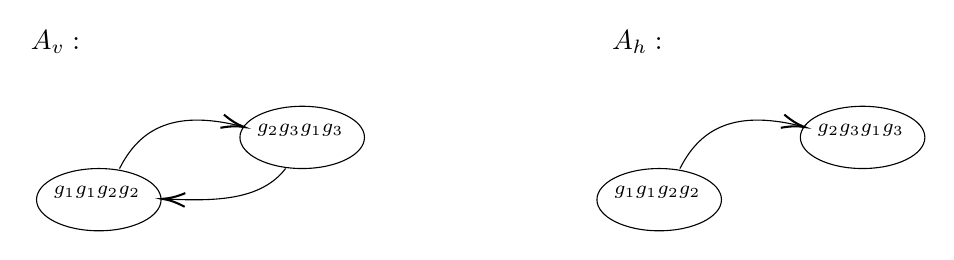
\begin{tikzpicture}[x=0.75pt,y=0.75pt,yscale=-1,xscale=1]
		%uncomment if require: \path (0,300); %set diagram left start at 0, and has height of 300
		
		%Shape: Ellipse [id:dp3480476979550604] 
		\draw   (140,115) .. controls (140,106.72) and (153.43,100) .. (170,100) .. controls (186.57,100) and (200,106.72) .. (200,115) .. controls (200,123.28) and (186.57,130) .. (170,130) .. controls (153.43,130) and (140,123.28) .. (140,115) -- cycle ;
		%Shape: Ellipse [id:dp9456474739758407] 
		\draw   (238,85) .. controls (238,76.72) and (251.43,70) .. (268,70) .. controls (284.57,70) and (298,76.72) .. (298,85) .. controls (298,93.28) and (284.57,100) .. (268,100) .. controls (251.43,100) and (238,93.28) .. (238,85) -- cycle ;
		%Shape: Ellipse [id:dp2502651910875927] 
		\draw   (410,115) .. controls (410,106.72) and (423.43,100) .. (440,100) .. controls (456.57,100) and (470,106.72) .. (470,115) .. controls (470,123.28) and (456.57,130) .. (440,130) .. controls (423.43,130) and (410,123.28) .. (410,115) -- cycle ;
		%Shape: Ellipse [id:dp3792185411216099] 
		\draw   (508,85) .. controls (508,76.72) and (521.43,70) .. (538,70) .. controls (554.57,70) and (568,76.72) .. (568,85) .. controls (568,93.28) and (554.57,100) .. (538,100) .. controls (521.43,100) and (508,93.28) .. (508,85) -- cycle ;
		%Curve Lines [id:da7858938212358939] 
		\draw    (180,100) .. controls (188.87,82.47) and (204.13,70.95) .. (238.42,79.59) ;
		\draw [shift={(240,80)}, rotate = 194.87] [color={rgb, 255:red, 0; green, 0; blue, 0 }  ][line width=0.75]    (10.93,-3.29) .. controls (6.95,-1.4) and (3.31,-0.3) .. (0,0) .. controls (3.31,0.3) and (6.95,1.4) .. (10.93,3.29)   ;
		%Curve Lines [id:da7351349882046846] 
		\draw    (260,100) .. controls (248.11,115.41) and (226.13,115.79) .. (202.43,114.69) ;
		\draw [shift={(200.6,114.6)}, rotate = 2.82] [color={rgb, 255:red, 0; green, 0; blue, 0 }  ][line width=0.75]    (10.93,-3.29) .. controls (6.95,-1.4) and (3.31,-0.3) .. (0,0) .. controls (3.31,0.3) and (6.95,1.4) .. (10.93,3.29)   ;
		%Curve Lines [id:da48287324374825746] 
		\draw    (450,100) .. controls (458.87,82.47) and (474.13,70.95) .. (508.42,79.59) ;
		\draw [shift={(510,80)}, rotate = 194.87] [color={rgb, 255:red, 0; green, 0; blue, 0 }  ][line width=0.75]    (10.93,-3.29) .. controls (6.95,-1.4) and (3.31,-0.3) .. (0,0) .. controls (3.31,0.3) and (6.95,1.4) .. (10.93,3.29)   ;
		
		% Text Node
		\draw (147,107.4) node [anchor=north west][inner sep=0.75pt]  [font=\scriptsize]  {$g_{1} g_{1} g_{2} g_{2}$};
		% Text Node
		\draw (245,77.4) node [anchor=north west][inner sep=0.75pt]  [font=\scriptsize]  {$g_{2} g_{3} g_{1} g_{3}$};
		% Text Node
		\draw (417,107.4) node [anchor=north west][inner sep=0.75pt]  [font=\scriptsize]  {$g_{1} g_{1} g_{2} g_{2}$};
		% Text Node
		\draw (515,77.4) node [anchor=north west][inner sep=0.75pt]  [font=\scriptsize]  {$g_{2} g_{3} g_{1} g_{3}$};
		% Text Node
		\draw (136,32.4) node [anchor=north west][inner sep=0.75pt]    {$A_{v} :$};
		% Text Node
		\draw (416,32.4) node [anchor=north west][inner sep=0.75pt]    {$A_{h} :$};
		
		
	\end{tikzpicture}
\end{figure}
	
	For the sake of completeness, assuming the possibility of rotation, then the set of possible tiles will be
	\begin{figure}[h!]
	\centering
	
	\tikzset{every picture/.style={line width=0.75pt}} %set default line width to 0.75pt        
	
	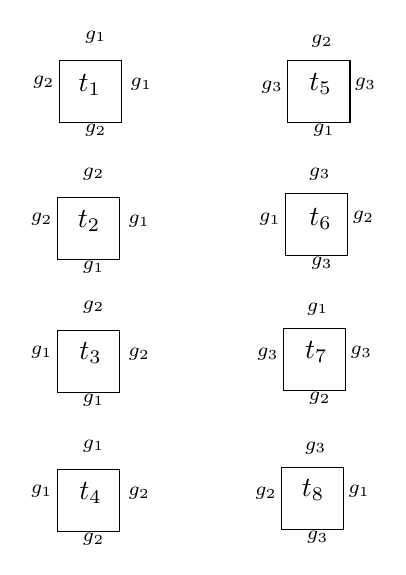
\begin{tikzpicture}[x=0.75pt,y=0.75pt,yscale=-1,xscale=1]
		%uncomment if require: \path (0,300); %set diagram left start at 0, and has height of 300
		
		%Shape: Square [id:dp22532401478603215] 
		\draw   (143,40) -- (173,40) -- (173,70) -- (143,70) -- cycle ;
		%Shape: Square [id:dp09979375032138338] 
		\draw   (253,40) -- (283,40) -- (283,70) -- (253,70) -- cycle ;
		%Shape: Square [id:dp3168351739514086] 
		\draw   (142,106) -- (172,106) -- (172,136) -- (142,136) -- cycle ;
		%Shape: Square [id:dp8233768301251638] 
		\draw   (142,170) -- (172,170) -- (172,200) -- (142,200) -- cycle ;
		%Shape: Square [id:dp752708971833606] 
		\draw   (142,237) -- (172,237) -- (172,267) -- (142,267) -- cycle ;
		%Shape: Square [id:dp5808750315542068] 
		\draw   (252,104) -- (282,104) -- (282,134) -- (252,134) -- cycle ;
		%Shape: Square [id:dp3802022570055066] 
		\draw   (251,169) -- (281,169) -- (281,199) -- (251,199) -- cycle ;
		%Shape: Square [id:dp6621336678331176] 
		\draw   (250,236) -- (280,236) -- (280,266) -- (250,266) -- cycle ;
		
		% Text Node
		\draw (154,24.4) node [anchor=north west][inner sep=0.75pt]  [font=\scriptsize]  {$g_{1}$};
		% Text Node
		\draw (176,47.4) node [anchor=north west][inner sep=0.75pt]  [font=\scriptsize]  {$g_{1}$};
		% Text Node
		\draw (154,69.4) node [anchor=north west][inner sep=0.75pt]  [font=\scriptsize]  {$g_{2}$};
		% Text Node
		\draw (129,46.4) node [anchor=north west][inner sep=0.75pt]  [font=\scriptsize]  {$g_{2}$};
		% Text Node
		\draw (263,26.4) node [anchor=north west][inner sep=0.75pt]  [font=\scriptsize]  {$g_{2}$};
		% Text Node
		\draw (284,47.4) node [anchor=north west][inner sep=0.75pt]  [font=\scriptsize]  {$g_{3}$};
		% Text Node
		\draw (264,69.4) node [anchor=north west][inner sep=0.75pt]  [font=\scriptsize]  {$g_{1}$};
		% Text Node
		\draw (239,48.4) node [anchor=north west][inner sep=0.75pt]  [font=\scriptsize]  {$g_{3}$};
		% Text Node
		\draw (153,90.4) node [anchor=north west][inner sep=0.75pt]  [font=\scriptsize]  {$g_{2}$};
		% Text Node
		\draw (175,113.4) node [anchor=north west][inner sep=0.75pt]  [font=\scriptsize]  {$g_{1}$};
		% Text Node
		\draw (153,135.4) node [anchor=north west][inner sep=0.75pt]  [font=\scriptsize]  {$g_{1}$};
		% Text Node
		\draw (128,112.4) node [anchor=north west][inner sep=0.75pt]  [font=\scriptsize]  {$g_{2}$};
		% Text Node
		\draw (153,154.4) node [anchor=north west][inner sep=0.75pt]  [font=\scriptsize]  {$g_{2}$};
		% Text Node
		\draw (175,177.4) node [anchor=north west][inner sep=0.75pt]  [font=\scriptsize]  {$g_{2}$};
		% Text Node
		\draw (153,199.4) node [anchor=north west][inner sep=0.75pt]  [font=\scriptsize]  {$g_{1}$};
		% Text Node
		\draw (128,176.4) node [anchor=north west][inner sep=0.75pt]  [font=\scriptsize]  {$g_{1}$};
		% Text Node
		\draw (153,221.4) node [anchor=north west][inner sep=0.75pt]  [font=\scriptsize]  {$g_{1}$};
		% Text Node
		\draw (175,244.4) node [anchor=north west][inner sep=0.75pt]  [font=\scriptsize]  {$g_{2}$};
		% Text Node
		\draw (153,266.4) node [anchor=north west][inner sep=0.75pt]  [font=\scriptsize]  {$g_{2}$};
		% Text Node
		\draw (128,243.4) node [anchor=north west][inner sep=0.75pt]  [font=\scriptsize]  {$g_{1}$};
		% Text Node
		\draw (262,90.4) node [anchor=north west][inner sep=0.75pt]  [font=\scriptsize]  {$g_{3}$};
		% Text Node
		\draw (283,111.4) node [anchor=north west][inner sep=0.75pt]  [font=\scriptsize]  {$g_{2}$};
		% Text Node
		\draw (263,133.4) node [anchor=north west][inner sep=0.75pt]  [font=\scriptsize]  {$g_{3}$};
		% Text Node
		\draw (238,112.4) node [anchor=north west][inner sep=0.75pt]  [font=\scriptsize]  {$g_{1}$};
		% Text Node
		\draw (261,155.4) node [anchor=north west][inner sep=0.75pt]  [font=\scriptsize]  {$g_{1}$};
		% Text Node
		\draw (282,176.4) node [anchor=north west][inner sep=0.75pt]  [font=\scriptsize]  {$g_{3}$};
		% Text Node
		\draw (262,198.4) node [anchor=north west][inner sep=0.75pt]  [font=\scriptsize]  {$g_{2}$};
		% Text Node
		\draw (237,177.4) node [anchor=north west][inner sep=0.75pt]  [font=\scriptsize]  {$g_{3}$};
		% Text Node
		\draw (260,222.4) node [anchor=north west][inner sep=0.75pt]  [font=\scriptsize]  {$g_{3}$};
		% Text Node
		\draw (281,243.4) node [anchor=north west][inner sep=0.75pt]  [font=\scriptsize]  {$g_{1}$};
		% Text Node
		\draw (261,265.4) node [anchor=north west][inner sep=0.75pt]  [font=\scriptsize]  {$g_{3}$};
		% Text Node
		\draw (236,244.4) node [anchor=north west][inner sep=0.75pt]  [font=\scriptsize]  {$g_{2}$};
		% Text Node
		\draw (151,45.4) node [anchor=north west][inner sep=0.75pt]    {$t_{1}$};
		% Text Node
		\draw (150.6,111) node [anchor=north west][inner sep=0.75pt]    {$t_{2}$};
		% Text Node
		\draw (151.4,174.6) node [anchor=north west][inner sep=0.75pt]    {$t_{3}$};
		% Text Node
		\draw (151.4,241.8) node [anchor=north west][inner sep=0.75pt]    {$t_{4}$};
		% Text Node
		\draw (262.2,45) node [anchor=north west][inner sep=0.75pt]    {$t_{5}$};
		% Text Node
		\draw (262.2,109.8) node [anchor=north west][inner sep=0.75pt]    {$t_{6}$};
		% Text Node
		\draw (260.2,174.2) node [anchor=north west][inner sep=0.75pt]    {$t_{7}$};
		% Text Node
		\draw (258.6,240.6) node [anchor=north west][inner sep=0.75pt]    {$t_{8}$};
		
		
	\end{tikzpicture}
\end{figure}
	
	where for the convenience we have assigned labels for each tile. The $ A_v $ graph for this set of tiles will be as the following graph, where the one on the left is $ A_v $ and the one on the right is $ A_h $.
	
	\begin{figure}[h!]
		\centering
		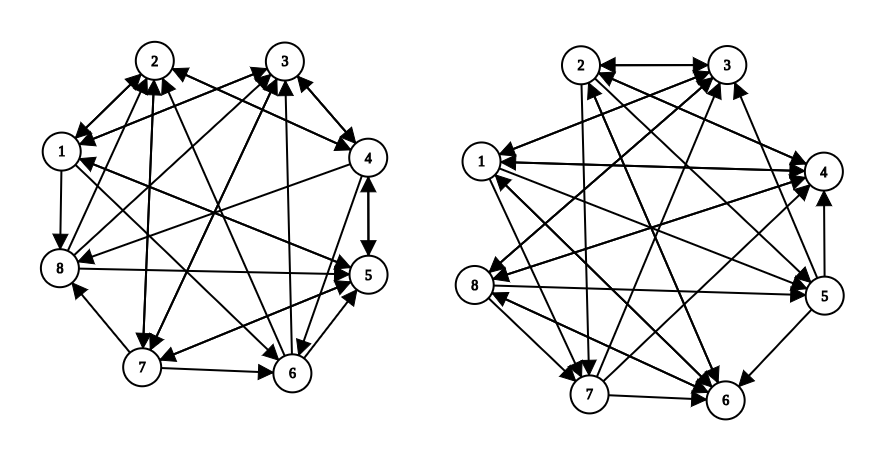
\includegraphics[width=0.5\linewidth]{images/A_vA_hwithRotation.png}
		\label{fig:graph}
	\end{figure}
	
	\FloatBarrier
	
	and one can do a similar computation to calculate the $ A_h $ graph.
	
	
	
	
	
	\section{Discussion}
	One important implication of this approach is that one can easily change the underlying grid structure with hexagonal grids, and etc.
	
	
	
\end{document}